\documentclass[landscape]{article}
\usepackage[margin=1in]{geometry}
\usepackage{graphicx}
\usepackage{hyperref}
\usepackage{multicol}

\newcommand{\bi}{\begin{itemize}}
\newcommand{\ii}{\item}
\newcommand{\ei}{\end{itemize}}

\newcommand{\sect}[1]{\newpage{\bf #1}}

\title{Notes on Using Blender for Games}
\author{Geoffrey Matthews}

\begin{document}

\maketitle

\LARGE
\sect{Textbook:}
\bi
\ii\url{http://www.cdschools.org/Page/455}
An excellent intro textbook.  Make sure you get the version for 
Blender 2.5/6.  For the game engine, read:
\begin{description}
\item[Chapter 1, The Blender Interface]
\item[Chapter 2, Working with Viewports]
\item[Chapter 3, Creating/Editing Objects]
\item[Chapter 4, Materials and Textures] 
You can only use image textures in the game engine,
  not any of Blender's generated textures.  See Chapter 22, also.
\item[Chapter 9, Animation Basics]
\item[Chapter 16, Armatures]
\item[Chapter 21, Game Engine Basics]
\item[Chapter 22, Game Engine Textures]
\end{description}
\ei

\sect{Beginning tutorials}
\bi
\ii \url{https://www.youtube.com/watch?v=tczC2URHRao}
Excellent 14-part series by Josh Beck, designed for 7th graders.

\ii \url{http://teachgames.wordpress.com/tutorials-blender/}
 Also has a platformer, and a short introduction in the 
tutorial notes.

\ii \url{https://www.youtube.com/watch?v=Mu_2IlsnK0k}

\ii\url{https://www.blender.org/support/tutorials/} Some interesting
game tutorials at the bottom.

  \ei

\sect{Physics tutorials}
\bi
\ii \url{https://www.youtube.com/watch?v=w3WG2W_Hi8I&index=2&list=PLMYtDzby1wdYpDbwoTuaXepAMZkxtEb6q}
\ei

\sect{Python tutorials}
\bi
\ii\url{http://www.cgmasters.net/free-tutorials/python-scripting/}

\ii\url{https://www.youtube.com/watch?v=CG4C7PZAqDQ&index=2&list=PLMYtDzby1wdZIHi203Xv5aoxestpF1zX9}

\ii\url{http://solarlune-gameup.blogspot.com/search/label/BGE%20Tutorials}
\ei

\sect{Platformer tutorials}
\bi
\ii\url{http://www.blendernation.com/2011/12/14/creating-a-platformer-in-the-blender-game-engine}
\ii\url{http://teachgames.wordpress.com/tutorials-blender/}
\ii\url{https://www.youtube.com/watch?v=SzwK7Ziwsao}
\ei

\sect{FPS tutorials}
\bi
\ii\url{http://blenderartists.org/forum/showthread.php?85219-BGE-FPS-Template-12-28-06}
\ii\url{http://blenderartists.org/forum/showthread.php?290771-How-to-make-an-FPS-game-in-Blender-2-6!-(HD-Video-tutorial)}

\ii\url{https://www.youtube.com/watch?v=d2BL9AxORec}
\ei



\sect{Use Blender 2.5 or higher}

\bi
\ii There was a huge change in Blender between 2.49 and 2.5
\ii 2.5 is MUCH better
\ii Only use tutorials for 2.5, 2.6, 2.7, ...
\ii Do not look at any tutorials for 2.49 or lower
\ii If the starting screen looks like this, with all the controls across
the bottom, DON'T USE IT:

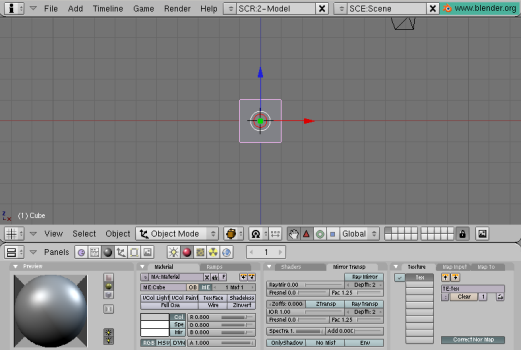
\includegraphics[scale=0.5]{oldblender.png}

\ei

\sect{Starting Blender Game Engine Development}
\begin{multicols}{2}
\bi
\ii Start blender
\ii Change rendering engine from {\bf Blender Render} to {\bf Blender Game}
\ii Expand right hand panel and lower panel.
\ii Change lower panel to game logic panel.
\ii Change Multitexture to GLSL in Render panel (tiny camera), Shading subpanel
\ii Save startup file
\ii Tools shelf
\ii 3D cursor
\ii Control-uparrow to maximize window
\ii Numpad views
\ii Mouse:
\bi
\ii Middle mouse: rotate
\ii Shift middle mouse:  translate
\ii Control middle mouse or Scroll:  zoom
\ei
\ii Objects:
\bi
\ii G: move (grab)
\ii R: rotate
\ii S: scale
\ei
\ii Multiple layouts
\ii Multiple scenes
\ii Use layers to simplify 
\ei
\end{multicols}

\sect{Add some objects}
\bi
\ii In the 3d window, press {\tt P} to play game
\ii Press {\tt esc} when done
\ii Move cube up
\ii In rendering properties (tiny camera), change Shading to GLSL
\ii Add a material and diffuse color 
(original cube already has material, pick color)
\ii Snap cursor to center (shift S)
\ii Add playing surface (shift A)
\ii Go to edit mode (tab)
\ii Scale by 10 (S then 10)
\ii Exit edit mode (tab)
\ii Add a material and diffuse color (buttons on right)
\ii Press {\tt P}
\ii Press esc
\ei

\sect{Add some behavior to the cube}

\bi
\ii Right-click the cube
\ii In the Game Logic panel create a keyboard sensor
\ii Set key to up arrow
\ii Create an and-controller
\ii Connect keyboard sensor
\ii Create a motion-actuator
\ii Connect and-controller
\ii Set motion to simple motion, local coordinates, change y location 0.1
\ii Make sure the L (local coordinates) button is pressed
\ii Generally best to regard y as forward, x as right, and z as up.
\ii In 3d window, press P
\ii Press up arrow.  Cube should move forward.
\ii Press esc
\ii Add left-arrow key sensor, connect to rotate z local 1
\ii Add right-arrow key sensor, connect to rotate z local -1
\ii Play game
\ei

\sect{Add some physics}

\bi
\ii Select (right click) the cube
\ii Go to physics button (bouncy ball)
\ii Change Static to Rigid Body
\ii Play game
\ii Walk off cliff
\ei

\sect{Add some balls}

\bi
\ii Add Collision bounds to cube
\ii Add two spheres
\ii Give them material and color
\ii Make them rigid bodies
\ii Play game, push spheres off cliff
\ii Edit spheres, check collision sphere
\ei

\sect{Using animations}

\bi
\ii Animate in animation screen
\ii Give animation a name
\ii Use actuator to play animation
\ii Remember to set first and last frames
\ei

\sect{Character modelling}

\bi
\ii Mirror modifier (Properties, modifiers under tiny wrench)
\ii Smooth shading (tool shelf, Tools: shading)
\ei

\sect{Character rigging}

\bi
\ii Set x-ray of armature (not mesh)
\ii E to extrude bone
\ii Turn on Armature Options X-Axis Mirror
\ii Shift-E to extrude mirror bones
\ii Parent mesh to armature, automatic weights
\ei

\sect{Character animation}
\bi
\ii Move armature in pose mode
\ii Select ALL bones
\ii Press I to insert pose
\ii Scroll to new time
\ii Copy/paste poses in mirror form
\ii Press I to insert pose
\ii Repeat
\ii Name animation to play in action actuator
\ii In game logic, attach action to armature, not mesh
\ei

\sect{Character textures}

\bi
\ii In Shading panel (tiny camera) change Shading to GLSL
\ii In texture panel make sure Material Texture is checked (three icons, sphere, sphere, tablecloth, check the middle one)
\ii Give object texture: Image (or Movie)
\ii Give texture NAME
\ii Give object new image
\ii Give image NAME
\ii In edit mode
\ii Select seam vertices
\ii Go to UV editing layout
\ii In image editor, select image NAME
\ii In 3d editor, edit mode, mark seam (tool shelf shading)
\ii Check seam to make sure you got it right
\ii Select all
\ii Unwrap object
\ii Change View to Paint (toolbar)
\ii Use image editor or external program
\ii If 3d window is in texture mode, can see edits in 3d
\ei

\sect{Skybox}

\bi
\ii Mark seam on cube to match your skybox
\ii Unwrap, UV map
\ii Set material to shadeless (Shading subpanel)
\ii Flip normals
\ii Scale 100
\ii Sky seam?
\ei

\sect{Game actions}
\bi
\ii End game, restart game
\ii Set scene
\ei

\sect{Miscellaneous}

\bi
\ii Shift-A to add something
\ii Shift-S to snap to somewhere
\ii Press control-A to apply rotations/scales/etc.
\ii Control-Z undo!
\ii Shift-control-Z redo (undo the undo)
\ii If you want to push a rigid body (e.g. sphere) around as the player,
use global coordinates in the motion actuator. 
\ei

\sect{Assets}
For models, rigs, textures, {\em etc.}
\bi
\ii\url{http://www.blendswap.com/}
\ii\url{https://cgcookie.com/blender/category/resources/}
\ii\url{http://www.blender-models.com/}
\ii\url{http://resources.blogscopia.com/}
\ii\url{http://www.makehuman.org/}
\ii\url{http://blenderartists.org} Some trailers of example games
\ii\url{http://www.rendertextures.com/}
\ei

\end{document}
